% orbital_resonance_lesson.tex
% Venus–Earth Orbital Resonance: The Rose and Pentagram of Venus
% Undergraduate Astronomy & Physics Lesson
% Compile with pdflatex or lualatex on Overleaf
% Author: Aaron Sells — STEM Tutoring
% ---------------------------------------------------------------

\documentclass[11pt,letterpaper]{article}

% ── Packages ──────────────────────────────────────────────────
\usepackage[margin=1in]{geometry}
\usepackage{amsmath,amssymb,amsthm}
\usepackage{physics}          % \dv, \pdv, \abs, \norm
\usepackage{siunitx}          % SI units
\usepackage{graphicx}
\usepackage{float}
\usepackage{booktabs}
\usepackage{enumitem}
\usepackage{hyperref}
\usepackage{cleveref}
\usepackage{xcolor}
\usepackage{tcolorbox}
\usepackage{tikz}
\usetikzlibrary{arrows.meta,calc,decorations.markings}
\usepackage{fancyhdr}
\usepackage{titlesec}
\usepackage{caption}

% ── Colors ────────────────────────────────────────────────────
\definecolor{venusGold}{HTML}{E8A838}
\definecolor{earthBlue}{HTML}{4488FF}
\definecolor{sunYellow}{HTML}{FFD700}
\definecolor{accentRed}{HTML}{CC3333}
\definecolor{noteGreen}{HTML}{2E8B57}

% ── Theorem environments ─────────────────────────────────────
\theoremstyle{definition}
\newtheorem{definition}{Definition}[section]
\newtheorem{example}{Example}[section]
\theoremstyle{plain}
\newtheorem{theorem}{Theorem}[section]
\newtheorem{proposition}{Proposition}[section]
\theoremstyle{remark}
\newtheorem{remark}{Remark}[section]

% ── Custom boxes ──────────────────────────────────────────────
\newtcolorbox{keyresult}{
  colback=earthBlue!8, colframe=earthBlue!70,
  title={\textbf{Key Result}}, fonttitle=\bfseries,
  arc=2mm, boxrule=0.8pt
}
\newtcolorbox{nasadata}{
  colback=venusGold!8, colframe=venusGold!70,
  title={\textbf{NASA/JPL Data}}, fonttitle=\bfseries,
  arc=2mm, boxrule=0.8pt
}
\newtcolorbox{historicalnote}{
  colback=noteGreen!8, colframe=noteGreen!70,
  title={\textbf{Historical Note}}, fonttitle=\bfseries,
  arc=2mm, boxrule=0.8pt
}
\newtcolorbox{physicsintuition}{
  colback=accentRed!6, colframe=accentRed!60,
  title={\textbf{Physical Intuition}}, fonttitle=\bfseries,
  arc=2mm, boxrule=0.8pt
}

% ── Header / Footer ──────────────────────────────────────────
\pagestyle{fancy}
\fancyhf{}
\lhead{\small Venus–Earth Orbital Resonance}
\rhead{\small Aaron Sells — STEM Tutoring}
\cfoot{\thepage}

% ── Title ─────────────────────────────────────────────────────
\title{%
  \vspace{-1cm}
  {\Huge\bfseries The Rose and Pentagram of Venus}\\[6pt]
  {\Large Venus–Earth Orbital Resonance\\
   and the Geometry of the Inner Solar System}\\[8pt]
  {\normalsize An Undergraduate Lesson in Orbital Mechanics,\\
   Coordinate Transformations, and Number Theory}
}
\author{%
  Aaron Sells\\
  \textit{STEM Tutoring — Lee's Summit, MO}
}
\date{November 2026}

\begin{document}
\maketitle
\thispagestyle{fancy}

% ══════════════════════════════════════════════════════════════
\begin{abstract}
If you track Venus's position from Earth's perspective for eight years,
something extraordinary emerges: a five-petaled flower pattern called the
\textit{Rose of Venus}, with the five closest-approach points forming a
near-perfect pentagram. This document develops the full mathematical
framework behind this phenomenon—from Kepler's laws and Keplerian orbital
mechanics, through synodic period derivation and heliocentric-to-geocentric
coordinate transformations, to the deep connection between the 13:8
orbital near-commensurability and Fibonacci numbers. All orbital elements
are drawn from NASA/JPL ephemeris data. The treatment is aimed at
undergraduate students in astronomy and physics.
\end{abstract}

\tableofcontents
\newpage

% ══════════════════════════════════════════════════════════════
\section{Introduction: A Cosmic Flower}
\label{sec:intro}

Follow Venus around the Earth for eight years.
Plot its position each day in Earth's reference frame—not the Sun's.
What appears is not a tangled mess but a strikingly symmetric
five-petaled flower, the \textbf{Rose of Venus}.

Connect the five points where Venus passes closest to Earth
(the \textit{inferior conjunctions}), and those five points form
a nearly perfect \textbf{pentagram}—a five-pointed star inscribed
in a circle.

\begin{historicalnote}
This pattern was known to Babylonian astronomers as early as
1500 BCE. The Maya tracked Venus's synodic cycle with extraordinary
precision. In Renaissance Europe, the pentagram of Venus was
linked to the golden ratio and to Pythagorean mysticism. It is
no accident that the planet of beauty traces geometry's most
beautiful polygon.
\end{historicalnote}

The root cause is a remarkable numerical coincidence:
\begin{keyresult}
In the time Earth completes \textbf{8 orbits} around the Sun,
Venus completes almost exactly \textbf{13 orbits}. The numbers
8, 13, and their difference 5 are consecutive Fibonacci numbers.
\end{keyresult}

This document will derive \textit{why} from first principles.


% ══════════════════════════════════════════════════════════════
\section{Foundations: Kepler's Laws of Planetary Motion}
\label{sec:kepler}

Johannes Kepler (1571–1630) distilled decades of Tycho Brahe's
observational data into three laws that govern planetary orbits.

% ── Kepler I ──────────────────────────────────────────────────
\subsection{First Law: The Law of Ellipses}

\begin{theorem}[Kepler's First Law]
Each planet moves in an \textbf{ellipse} with the Sun at one focus.
\end{theorem}

An ellipse with semi-major axis $a$ and eccentricity $e$
($0 \le e < 1$) has the polar equation (focus at origin):
\begin{equation}
  r(\nu) = \frac{a(1 - e^2)}{1 + e\cos\nu}
  \label{eq:ellipse}
\end{equation}
where $\nu$ is the \textbf{true anomaly}—the angle measured from
perihelion (closest approach to the Sun).

\begin{nasadata}
\begin{center}
\begin{tabular}{lcc}
  \toprule
  \textbf{Parameter} & \textbf{Venus} & \textbf{Earth} \\
  \midrule
  Semi-major axis $a$ (AU) & 0.72333199 & 1.00000011 \\
  Eccentricity $e$         & 0.00677323 & 0.01671022 \\
  Inclination $i$ (\si{\degree}) & 3.39471 & 0.00005 \\
  Orbital period $T$ (days) & 224.701 & 365.256 \\
  \bottomrule
\end{tabular}
\end{center}
\vspace{4pt}
\small Source: NASA/JPL NSSDC Planetary Fact Sheet (J2000 epoch)
\end{nasadata}

\begin{physicsintuition}
Venus has one of the most circular orbits in the solar system,
with $e_V = 0.0068$—its distance from the Sun varies by only
$\pm 0.68\%$. Earth's orbit is more eccentric ($e_E = 0.0167$),
varying by $\pm 1.67\%$. These small eccentricities are what
make the rose pattern so nearly symmetric—if either orbit were
highly elliptical, the petals would be lopsided.
\end{physicsintuition}


% ── Kepler II ─────────────────────────────────────────────────
\subsection{Second Law: The Law of Equal Areas}

\begin{theorem}[Kepler's Second Law]
A line joining a planet and the Sun sweeps out \textbf{equal areas
in equal times}.
\end{theorem}

Equivalently, the \textit{areal velocity} is constant:
\begin{equation}
  \dv{A}{t} = \frac{1}{2}\,r^2\,\dv{\nu}{t} = \text{const.}
  \label{eq:areal}
\end{equation}

This is a direct consequence of conservation of angular momentum
$L = m\,r^2\,\dot{\nu}$. At perihelion ($r$ smallest), the planet
moves fastest ($\dot{\nu}$ largest); at aphelion, slowest.


% ── Kepler III ────────────────────────────────────────────────
\subsection{Third Law: The Harmonic Law}

\begin{theorem}[Kepler's Third Law]
The square of the orbital period is proportional to the cube of the
semi-major axis:
\begin{equation}
  T^2 = \frac{4\pi^2}{G\,M_\odot}\,a^3
  \label{eq:kepler3}
\end{equation}
\end{theorem}

For two planets orbiting the same star, this gives the ratio:
\begin{equation}
  \frac{T_1^2}{T_2^2} = \frac{a_1^3}{a_2^3}
  \label{eq:kepler3ratio}
\end{equation}

\begin{example}[Verification with NASA data]
\[
  \frac{T_E^2}{T_V^2}
  = \frac{365.256^2}{224.701^2}
  = \frac{133\,411.9}{50\,470.5}
  = 2.6430
\]
\[
  \frac{a_E^3}{a_V^3}
  = \frac{1.00000011^3}{0.72333199^3}
  = \frac{1.0000}{0.37854}
  = 2.6417
\]
Agreement to 0.05\%—well within the precision of tabulated elements.
\end{example}


% ══════════════════════════════════════════════════════════════
\section{The Keplerian Orbital Mechanics Engine}
\label{sec:keplerian}

To compute a planet's position at any time $t$, we solve the
\textbf{Kepler problem}: given the orbital elements $(a, e, T)$
and an initial mean longitude $L_0$, find the heliocentric
Cartesian coordinates $(x, y)$.

\subsection{Mean Anomaly}

The \textbf{mean anomaly} $M$ is a fictitious angle that increases
uniformly with time:
\begin{equation}
  M(t) = M_0 + n\,(t - t_0), \qquad
  n = \frac{2\pi}{T}
  \label{eq:mean_anomaly}
\end{equation}
where $n$ is the \textbf{mean motion} (angular velocity of a
hypothetical circular orbit with the same period).

The initial mean anomaly $M_0$ is derived from the mean longitude
$L_0$ and longitude of perihelion $\varpi$:
\begin{equation}
  M_0 = L_0 - \varpi
  \label{eq:M0}
\end{equation}

\subsection{Kepler's Equation and Eccentric Anomaly}

The connection between $M$ (which we know) and the planet's actual
position requires solving \textbf{Kepler's equation}:

\begin{equation}
  \boxed{M = E - e\sin E}
  \label{eq:kepler_eqn}
\end{equation}

where $E$ is the \textbf{eccentric anomaly}. This transcendental
equation cannot be solved in closed form—it requires numerical
iteration.

\subsubsection{Newton–Raphson Method}

Define $f(E) = E - e\sin E - M$. Then $f'(E) = 1 - e\cos E$, and
Newton's iteration is:
\begin{equation}
  E_{n+1} = E_n - \frac{E_n - e\sin E_n - M}{1 - e\cos E_n}
  \label{eq:newton}
\end{equation}

\begin{physicsintuition}
For nearly circular orbits like Venus ($e = 0.0068$), Kepler's
equation is ``easy''—$E \approx M$ is already a good starting guess,
and Newton–Raphson converges in 2--3 iterations to machine precision.
For high-eccentricity orbits (comets with $e \to 1$), more
sophisticated starting guesses (such as Danby's cubic) are needed.
\end{physicsintuition}

\subsubsection{Danby's Starting Guess}

A refined initial estimate due to Danby (1988):
\begin{equation}
  E_0 = M + e\,\sin M + \frac{e^2}{2}\sin 2M
  \label{eq:danby}
\end{equation}
This third-order approximation is accurate to $\mathcal{O}(e^3)$ and
is especially useful when $e$ is not negligible.


\subsection{True Anomaly}

From the eccentric anomaly $E$, the \textbf{true anomaly} $\nu$
(the actual angular position) is:
\begin{equation}
  \nu = 2\arctan\!\left(
    \sqrt{\frac{1+e}{1-e}}\;\tan\frac{E}{2}
  \right)
  \label{eq:true_anomaly}
\end{equation}

\subsection{Heliocentric Distance and Cartesian Coordinates}

The heliocentric distance is:
\begin{equation}
  r = a\,(1 - e\cos E)
  \label{eq:helio_distance}
\end{equation}

Combining with the true anomaly, the heliocentric Cartesian
coordinates (in the orbital plane) are:
\begin{equation}
  \begin{pmatrix} x \\ y \end{pmatrix}
  = r \begin{pmatrix} \cos(\nu + \varpi) \\ \sin(\nu + \varpi) \end{pmatrix}
  \label{eq:helio_cartesian}
\end{equation}

where $\varpi$ is the longitude of perihelion.

\subsection{The Complete Pipeline}

\begin{equation}
  t \;\xrightarrow{\text{Eq.~\ref{eq:mean_anomaly}}}\;
  M \;\xrightarrow{\text{Eq.~\ref{eq:kepler_eqn}}}\;
  E \;\xrightarrow{\text{Eq.~\ref{eq:true_anomaly}}}\;
  \nu \;\xrightarrow{\text{Eq.~\ref{eq:helio_cartesian}}}\;
  (x,y)_{\text{helio}}
  \label{eq:pipeline}
\end{equation}

This pipeline is the core ``engine'' that powers every frame of our
Manim animation.


% ══════════════════════════════════════════════════════════════
\section{The Synodic Period}
\label{sec:synodic}

\subsection{Definition and Derivation}

The \textbf{synodic period} $P_{\text{syn}}$ is the time between
successive identical configurations of two planets as seen from one
of them—e.g., the time between consecutive inferior conjunctions
of Venus (when Venus passes between Earth and the Sun).

\begin{definition}[Synodic Period]
The angular velocities are $\omega_V = 2\pi/T_V$ and
$\omega_E = 2\pi/T_E$. Since Venus is faster (inner orbit),
the \textit{relative} angular velocity is:
\begin{equation}
  \omega_{\text{rel}} = \omega_V - \omega_E
  = \frac{2\pi}{T_V} - \frac{2\pi}{T_E}
\end{equation}

One complete ``lap'' (Venus gaining $2\pi$ on Earth) takes:
\begin{equation}
  \boxed{
    \frac{1}{P_{\text{syn}}}
    = \frac{1}{T_V} - \frac{1}{T_E}
  }
  \label{eq:synodic}
\end{equation}
\end{definition}

\begin{keyresult}
\[
  \frac{1}{P_{\text{syn}}}
  = \frac{1}{224.701} - \frac{1}{365.256}
  = 0.004451 - 0.002738
  = 0.001713\;\text{day}^{-1}
\]
\[
  P_{\text{syn}} = \frac{1}{0.001713} \approx \SI{583.9}{days}
  \approx \SI{1.599}{years}
\]
\end{keyresult}


\subsection{Physical Meaning}

Each synodic period contains one complete ``dance cycle'':
\begin{enumerate}[nosep]
  \item Venus overtakes Earth (inferior conjunction — closest)
  \item Venus races ahead as a ``morning star''
  \item Venus reaches maximum elongation west
  \item Venus passes behind the Sun (superior conjunction — farthest)
  \item Venus reappears as an ``evening star''
  \item Venus reaches maximum elongation east
  \item Venus approaches Earth again for the next inferior conjunction
\end{enumerate}

This cycle traces \textbf{one petal} of the Rose of Venus in the
geocentric frame.


% ══════════════════════════════════════════════════════════════
\section{Coordinate Transformations: Heliocentric to Geocentric}
\label{sec:transform}

The ``rose'' pattern is invisible in heliocentric coordinates—it
lives in the \textbf{geocentric frame}, where Earth is the fixed
origin.

\subsection{The Transformation}

This is simply vector subtraction. If $\vb{r}_V(t)$ and
$\vb{r}_E(t)$ are the heliocentric position vectors of Venus
and Earth:

\begin{equation}
  \boxed{
    \vb{r}_{V,\text{geo}}(t)
    = \vb{r}_V(t) - \vb{r}_E(t)
  }
  \label{eq:geocentric}
\end{equation}

\begin{physicsintuition}
This is the same transformation you use in everyday life:
to find where your friend is \textit{relative to you},
subtract your position from theirs. The fact that it produces
such stunning geometry is a consequence of the near-rational
period ratio, not of any special physics in the transformation
itself.
\end{physicsintuition}

\subsection{Computation Pipeline}

For each time step $t$:
\begin{enumerate}[nosep]
  \item Solve the Kepler problem for Venus $\to (x_V, y_V)$
  \item Solve the Kepler problem for Earth $\to (x_E, y_E)$
  \item Subtract: $(x_{V,\text{geo}},\, y_{V,\text{geo}})
        = (x_V - x_E,\, y_V - y_E)$
\end{enumerate}

This is evaluated at thousands of time steps to trace the
continuous geocentric path.


% ══════════════════════════════════════════════════════════════
\section{The 13:8 Near-Commensurability}
\label{sec:resonance}

\subsection{The Period Ratio}

\begin{equation}
  \frac{T_E}{T_V}
  = \frac{365.256}{224.701}
  = 1.62554\ldots
  \approx \frac{13}{8} = 1.625
  \label{eq:ratio}
\end{equation}

The agreement is striking: $1.62554$ vs.\ $1.625$, a discrepancy
of only \textbf{0.033\%}.

\subsection{What ``Near-Commensurability'' Means}

If the ratio were \textit{exactly} $13/8$, then after 8 Earth
years Venus would return to \textit{precisely} its starting
configuration, and the rose pattern would close perfectly. The
slight deviation means the pattern \textit{almost} closes—each
8-year cycle, the entire pattern drifts by about $2.55°$ (called
\textbf{precession} of the rose).

\begin{keyresult}
In 8 Earth years ($= 2922.05$ days):
\begin{itemize}[nosep]
  \item Venus completes $2922.05 / 224.701 = 13.0043$ orbits
  \item That extra $0.0043$ of an orbit $= 0.0043 \times 360° = 1.55°$ of Venus longitude
  \item The pattern drifts $\approx 2.55°$ retrograde per 8-year cycle
\end{itemize}
Full-pattern repetition period: $360° / 2.55° \approx 141$ cycles
$\approx 1130$ years.
\end{keyresult}

\begin{remark}
This is a \textbf{near-commensurability}, not a true orbital
resonance. True resonances (such as the 2:1 resonance between
Io and Europa) involve gravitational locking. Venus and Earth
do not gravitationally lock each other—the near-integer ratio
is a coincidence of the solar system's initial conditions.
\end{remark}

\subsection{Counting the Petals}

\begin{proposition}
If $T_E / T_V \approx p/q$ (in lowest terms), the geocentric
path has $p - q$ petals and $p - q$ inferior conjunctions per
cycle.
\end{proposition}

\begin{proof}
In $q$ Earth years, Venus completes $p$ orbits. The number of
times Venus ``laps'' Earth is $p - q$, since each lap corresponds
to one synodic cycle (one inferior conjunction, one petal).
For Venus--Earth: $13 - 8 = \mathbf{5}$ petals.
\end{proof}


% ══════════════════════════════════════════════════════════════
\section{The Pentagram of Venus}
\label{sec:pentagram}

\subsection{Inferior Conjunction Geometry}

Each inferior conjunction occurs when Venus passes between Earth
and the Sun. These 5 events are spaced by one synodic period
($\approx 583.9$ days) but separated in \textit{ecliptic longitude}
by:
\begin{equation}
  \Delta\lambda
  = P_{\text{syn}} \times \omega_E
  = 583.9 \times \frac{360°}{365.256}
  \approx 575.3°
  \equiv 575.3° - 360° = 215.3°
  \label{eq:conj_separation}
\end{equation}

Converting to the fraction of a circle that isn't traversed:
$360° - 215.3° = 144.7° \approx 144°$.

\begin{keyresult}
The 5 inferior conjunctions are separated by approximately
$\mathbf{144°}$ of ecliptic longitude—close to the
interior angle of a regular pentagon ($108°$) crossed with
the central angle of a pentagram ($144° = 360° \times 2/5$).
Connecting consecutive conjunctions produces a
\textbf{pentagram} inscribed in the zodiac.
\end{keyresult}

\subsection{Why $144°$?}

\begin{equation}
  \frac{P_{\text{syn}}}{T_E}
  = \frac{583.9}{365.256}
  = 1.5984 \approx \frac{8}{5}
\end{equation}

Each synodic period, Earth advances $1.5984$ full orbits, i.e.,
$0.5984$ of an orbit past the integer. In degrees:
$0.5984 \times 360° \approx 215.4°$. The ``shortfall'' from a
full circle is $360° - 215.4° = 144.6° \approx 2/5$ of $360°$.

This means consecutive conjunctions skip 2 out of 5 ``slots''
around the circle—exactly the rule for drawing a pentagram
(connect every second vertex of a regular pentagon).

\subsection{The Pentagram and the Pentagon}

\begin{center}
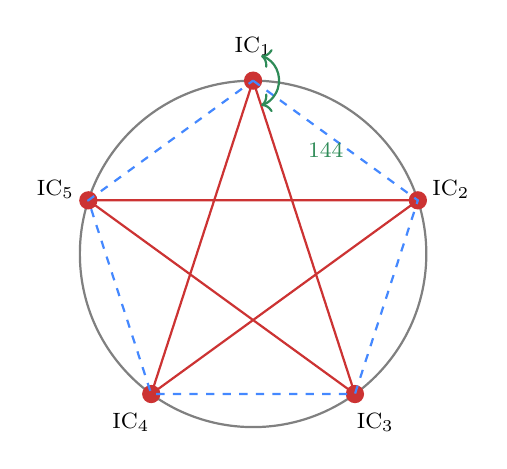
\begin{tikzpicture}[scale=2.2]
  % Circle
  \draw[gray,thick] (0,0) circle (1);
  % 5 conjunction points (starting at top, going clockwise by 144°)
  \foreach \i/\label in {0/IC$_1$, 1/IC$_2$, 2/IC$_3$, 3/IC$_4$, 4/IC$_5$} {
    \coordinate (P\i) at ({90 - \i*72}:1);
    \fill[accentRed] (P\i) circle (1.5pt);
    \node[font=\footnotesize] at ({90 - \i*72}:1.2) {\label};
  }
  % Pentagram (connect every 2nd point)
  \draw[accentRed,thick]
    (P0) -- (P2) -- (P4) -- (P1) -- (P3) -- cycle;
  % Pentagon
  \draw[earthBlue,thick,dashed]
    (P0) -- (P1) -- (P2) -- (P3) -- (P4) -- cycle;
  % Annotations
  \draw[<->,noteGreen,thick] ([shift={(72:0.15)}]P0)
    arc[start angle=72,end angle={72-144},radius=0.15];
  \node[noteGreen,font=\footnotesize] at (0.42,0.6) {$144°$};
\end{tikzpicture}
\end{center}
\captionof{figure}{The 5 inferior conjunctions (red dots) form a
  regular pentagon (blue dashed). Connecting them in temporal order
  (red solid) draws a pentagram. Consecutive conjunctions subtend
  $\approx 144°$.}


% ══════════════════════════════════════════════════════════════
\section{The Golden Ratio and Fibonacci Connection}
\label{sec:golden}

\subsection{Fibonacci Numbers in the Solar System}

The three numbers governing Venus--Earth geometry are:
\[
  5, \quad 8, \quad 13
\]
These are \textit{consecutive Fibonacci numbers}
($F_5 = 5$, $F_6 = 8$, $F_7 = 13$), where each is the sum of
the two before it: $5 + 8 = 13$.

\subsection{The Golden Ratio}

The golden ratio is:
\begin{equation}
  \varphi = \frac{1 + \sqrt{5}}{2} = 1.6180339887\ldots
  \label{eq:golden}
\end{equation}

The ratio of consecutive Fibonacci numbers converges to $\varphi$:
\begin{equation}
  \frac{13}{8} = 1.625,
  \qquad
  \varphi = 1.6180\ldots,
  \qquad
  \text{difference} = 0.43\%
  \label{eq:fib_golden}
\end{equation}

\begin{physicsintuition}
The golden ratio appears here \textit{because} of the Fibonacci
structure. The Venus--Earth period ratio happens to land near
$13/8$, a Fibonacci ratio, which is close to $\varphi$. This is
a numerical coincidence of initial conditions, not a deep physical
law—but it explains why the pentagram (the geometric figure most
intimately connected to $\varphi$) appears in Venus's geocentric
path.
\end{physicsintuition}

\subsection{The Golden Ratio in the Pentagram}

The diagonals of a regular pentagon divide each other in the
golden ratio:
\begin{equation}
  \frac{\text{diagonal}}{\text{side}} = \varphi = \frac{1+\sqrt{5}}{2}
\end{equation}

This is why the same number, $\varphi$, connects:
\begin{itemize}[nosep]
  \item The Venus--Earth period ratio ($\approx 13/8 \approx \varphi$)
  \item The number of petals ($13 - 8 = 5$)
  \item The angular separation of conjunctions ($144° = 2/5 \times 360°$)
  \item The geometry of the pentagram the conjunctions trace
\end{itemize}


% ══════════════════════════════════════════════════════════════
\section{The Rose Pattern: Parametric Description}
\label{sec:rose}

\subsection{Simplified Model (Circular Orbits)}

For intuition, consider a simplified model where both orbits are
perfect circles ($e = 0$). Then Venus's geocentric path is
described by the parametric equations:
\begin{equation}
  \begin{aligned}
    x(t) &= a_V \cos(\omega_V t) - a_E \cos(\omega_E t) \\
    y(t) &= a_V \sin(\omega_V t) - a_E \sin(\omega_E t)
  \end{aligned}
  \label{eq:circular_rose}
\end{equation}

This is a \textbf{hypotrochoid}—a curve generated by one circle
rolling inside another. The key parameter is the frequency ratio
$\omega_V / \omega_E = T_E / T_V \approx 13/8$.

\subsection{Rose Curves}

The standard polar rose curve $r = \cos(k\theta)$ has:
\begin{itemize}[nosep]
  \item $k$ petals if $k$ is odd
  \item $2k$ petals if $k$ is even
  \item $p - q$ petals if $k = p/q$ in lowest terms
\end{itemize}

For Venus--Earth, the ``effective $k$'' gives $13 - 8 = 5$ petals.

\subsection{Full Keplerian Model}

The actual pattern uses the full Keplerian orbits from
\cref{sec:keplerian}, including:
\begin{itemize}[nosep]
  \item Non-zero eccentricity (petals slightly asymmetric)
  \item Longitude of perihelion offsets (pattern rotation)
  \item Non-exact commensurability (pattern drift)
\end{itemize}

The Manim animation accompanying this lesson uses the full
Keplerian model with NASA/JPL orbital elements.


% ══════════════════════════════════════════════════════════════
\section{Historical and Cultural Significance}
\label{sec:history}

\begin{historicalnote}
\textbf{Babylonian astronomy} (c.\ 1500 BCE): Tablets record Venus's
synodic cycle; the \textit{Venus Tablet of Ammisaduqa} (c.\ 1650 BCE)
contains the earliest known Venus observations.

\textbf{Mayan astronomy}: The Dresden Codex devotes 6 pages to Venus's
synodic cycle, using $584$ days (remarkably close to the actual
$583.9$). Venus governed the timing of warfare and ritual.

\textbf{Pythagorean tradition}: The pentagram was the symbol of the
Pythagorean brotherhood, associated with health (\textit{hygieia})
and harmony. Its connection to the golden ratio was central to their
philosophy of number.

\textbf{Copernicus and Kepler}: The geometric regularity of Venus's
geocentric path was one of many observations that the Copernican
heliocentric model could explain more simply than Ptolemy's epicycles.
Kepler himself was deeply moved by the ``harmonies'' of planetary
motion.
\end{historicalnote}


% ══════════════════════════════════════════════════════════════
\section{Summary of Key Equations}
\label{sec:summary}

\begin{center}
\renewcommand{\arraystretch}{1.4}
\begin{tabular}{lll}
  \toprule
  \textbf{Concept} & \textbf{Equation} & \textbf{Ref.} \\
  \midrule
  Elliptical orbit     & $r = a(1-e^2)/(1+e\cos\nu)$
                       & (\ref{eq:ellipse}) \\
  Kepler III           & $T^2 = 4\pi^2 a^3 / (GM_\odot)$
                       & (\ref{eq:kepler3}) \\
  Mean anomaly         & $M = M_0 + (2\pi/T)(t-t_0)$
                       & (\ref{eq:mean_anomaly}) \\
  Kepler's equation    & $M = E - e\sin E$
                       & (\ref{eq:kepler_eqn}) \\
  Newton–Raphson       & $E_{n+1} = E_n - f(E_n)/f'(E_n)$
                       & (\ref{eq:newton}) \\
  True anomaly         & $\nu = 2\arctan\!\bigl[\sqrt{(1\!+\!e)/(1\!-\!e)}\,\tan(E/2)\bigr]$
                       & (\ref{eq:true_anomaly}) \\
  Synodic period       & $1/P_\text{syn} = 1/T_V - 1/T_E$
                       & (\ref{eq:synodic}) \\
  Geocentric transform & $\vb{r}_{V,\text{geo}} = \vb{r}_V - \vb{r}_E$
                       & (\ref{eq:geocentric}) \\
  Period ratio         & $T_E/T_V = 1.6255 \approx 13/8$
                       & (\ref{eq:ratio}) \\
  Golden ratio         & $\varphi = (1+\sqrt{5})/2 = 1.618\ldots$
                       & (\ref{eq:golden}) \\
  \bottomrule
\end{tabular}
\end{center}


% ══════════════════════════════════════════════════════════════
\section{Glossary}
\label{sec:glossary}

\begin{description}[style=nextline,leftmargin=3cm]
  \item[Aphelion] Point in an orbit farthest from the Sun.
  \item[Eccentric anomaly ($E$)] Auxiliary angle used in solving the Kepler problem.
  \item[Eccentricity ($e$)] Measure of orbital elongation; $e=0$ is a circle.
  \item[Geocentric] Referenced to Earth as the origin.
  \item[Heliocentric] Referenced to the Sun as the origin.
  \item[Inferior conjunction] Configuration where an inner planet passes between Earth and the Sun.
  \item[Mean anomaly ($M$)] Uniformly increasing angle proportional to elapsed time.
  \item[Mean motion ($n$)] Angular velocity of a fictitious circular orbit; $n = 2\pi/T$.
  \item[Near-commensurability] Two periods whose ratio is close to a ratio of small integers.
  \item[Perihelion] Point in an orbit closest to the Sun.
  \item[Resonance] Gravitational locking of orbital periods at a rational ratio.
  \item[Semi-major axis ($a$)] Half the longest diameter of an ellipse.
  \item[Superior conjunction] Configuration where a planet is on the far side of the Sun from Earth.
  \item[Synodic period] Time between successive identical planet configurations as seen from Earth.
  \item[True anomaly ($\nu$)] Actual angular position measured from perihelion.
\end{description}


% ══════════════════════════════════════════════════════════════
\section*{References}

\begin{enumerate}[label={[\arabic*]},nosep]
  \item NASA/GSFC NSSDC Planetary Fact Sheet:
    \url{https://nssdc.gsfc.nasa.gov/planetary/factsheet/}
  \item Standish, E.\ M.\ (1992).
    ``Keplerian Elements for Approximate Positions of the Major Planets.''
    JPL Solar System Dynamics.
  \item Murray, C.\ D.\ \& Dermott, S.\ F.\ (1999).
    \textit{Solar System Dynamics}. Cambridge University Press.
  \item Danby, J.\ M.\ A.\ (1988).
    \textit{Fundamentals of Celestial Mechanics}, 2nd ed.
    Willmann-Bell.
  \item Meeus, J.\ (1991).
    \textit{Astronomical Algorithms}. Willmann-Bell.
  \item ``Follow Venus Around Earth for 8 Years and It Draws a Flower.''
    Cosmic Starships, YouTube.
    \url{https://youtube.com/shorts/8f1jdaS2J00}
\end{enumerate}

\end{document}
